\documentclass[12pt,oneside,openright]{report}

\usepackage[utf8]{inputenc}
\usepackage[scaled]{helvet}
\usepackage{subcaption} % Add the subcaption package for subfigures
\usepackage{dirtytalk} %quoting package
\renewcommand\familydefault{\sfdefault} 
\usepackage[T1]{fontenc}
\usepackage{fancyhdr,xcolor}

\usepackage{graphicx} % Add the graphicx package for including images
\usepackage{geometry}
\usepackage{amsmath} % Add this line to your LaTeX preamble to use \text
\usepackage{changepage}
\usepackage{pdfpages}
\usepackage{afterpage}
\usepackage{caption}
\usepackage{float}
\usepackage{xcolor}

\usepackage[style=authoryear,backend=biber]{biblatex}
\addbibresource{bibliog.bib}
\usepackage[colorlinks=true,linkcolor=black,anchorcolor=black,citecolor=black,filecolor=black,menucolor=black,runcolor=black,urlcolor=black]{hyperref}\usepackage{graphicx}
\usepackage{adjustbox}
\geometry{
  a4paper,
  left=20mm,
  right=20mm,
  top=3cm,
  headheight=4cm,
  bottom=3.5cm,
  footskip=3cm
}

\renewcommand*{\bibfont}{\footnotesize}

\newcommand{\changefont}{
    \fontsize{18}{16}\selectfont
}
\definecolor{boxcl}{HTML}{1188BB}
\definecolor{tubred}{HTML}{1188BB}



\begin{document}

\begin{titlepage}
    \centering
    % Include the image with a width of one-third of the page
    
\includegraphics[width=0.5\textwidth]{Hu-logo.png}
    \vspace{2cm}
    
    {\huge \textbf{Multisensory Integration in Virtual Reality: Effects of Passive Haptic Stimulation}\par}
    \vspace{2cm}
    {\LARGE Master Thesis\par}
    \vspace{0.5cm}
    {\textbf{submitted in fulfilment of the requirements for the degree}\par}
    Master of Science (M.Sc.)\par
    {\textbf{in the master's program ``Mind and Brain''}\par}
    \vspace{1.5cm}
    {\textbf{Humboldt-Universität zu Berlin}\par}
    {\textbf{Berlin School of Mind and Brain}\par}
    \vfill
    \raggedright
    \begin{tabular}{ll}
        \textbf{Handed in by}: & Benjamin Dupré \\
        \textbf{Date of birth:} & 26.04.1986\\
       \textbf{ Address:} & Hoppestraße 16, 13409, Berlin \\
    \end{tabular}
    \vfill
    \begin{tabular}{ll}
        \textbf{1. Supervisor:}& Dr. Michael Gaebler \\
        \textbf{2. Supervisor:}& Professor Dr. Arno Villringer  \\
    \end{tabular}
    \vfill
    {Berlin, \today \par}
\end{titlepage}

\newpage
%\thispagestyle{empty}
\section*{\centering Acknowledgments}

\begin{adjustwidth}{1cm}{1cm}
%\begin{center}

I would like to express my sincere gratitude to Dr. Michael Gaebler for his constant advice.  To Prof. Dr. Arno Villringer for his support in making this thesis possible. Many thanks to Max Hellrigel-Holderbaum for his friendly editing and references, as well as to Dr. Zeynep Akbal and Dr. Tim Julian Möller for generously sharing their expertise and time.

I am deeply grateful for the support provided by the Max-Planck Institute, specifically from Dr. Zeynep Akbal and Prof. Dr. Arno Villringer (NRO-228 - Study-DB (0218807)).
    
%\end{center}
\end{adjustwidth}

\clearpage

\section*{1. Introduction}
\subsubsection*{Immersive Virtual Reality evokes psychophysical reactions}

Immersive Virtual Reality (IVR) is a computer-generated environment that simulates real-world interactions through electronic equipment. In IVR, visual, auditory, and tactile signals can be replaced with computer-mediated inputs, enveloping individuals in a virtual environment. In other words, it gives the user a sense of physical presence within a digitally constructed world. Presence, in this context, refers to the sensation of being within the virtual environment rather than the physical space one occupies. It is precisely this 'suspension of reality' what makes immersive experiences able to elicit a range of responses from individuals. This, responses span between emotional, behavioural, and psychophysical reactions \parencite{SanchezVives2005FromPT}. We will understand for psychphysical reactions the subjective perceptual response to a stimulus with described physical characteristics. All of these responses, akin to those elicited by traditional media such as theatre or films, often exhibit heightened intensity within IVR. Thus, making it a compelling tool for investigating human behaviour, cognition, and perception. 

IVR can be seen as a continuation of a long psychophysical tradition that attempts to interfere with our perception to clarify its underlying mechanism. In the past for example, lenses or prisms have been used to invert visual perception of orientation to study the visual properties of the cortex \parencite{deGelder2018VirtualRA} and IVR would be somewhere along this lines. Nonetheless, if we are to use IVR as a tool to do psychophysical perception studies, many will question its validity and how it compares to real-life. While this issue is in part philosophical and extends beyond the scope of this thesis, recent empirical research offers insights into the comparison of IVR, real-life and computer base experimental setups for psychophysical and other relevant markers.

How comparable is IVR to what we experience in real-life or in current experimental setups? A recent study took on these questions by comparing three experimental set-ups: One in physical reality, another in virtual reality and the last one displayed on a computer screen and keyboard setup. The participants needed to climb up into a firefighter hydraulic platform presented to them via the three above mentioned setups, while the authors looked at various markers like electrophysiological, physiological, and subjective responses (e.g. ECG, ECG, Surveys). What they found was that our brain and body seem to react similarly in both real-life and virtual situations. Specifically, alpha- and theta-band oscillations, heart rate variability, indexed vigilance, and anxiety were barely indistinguishable between VR and real-life. While they differed significantly from computer screen display setup. Sensory processing, as reflected by beta-band oscillations, exhibits a different pattern for all conditions, indicating further room for improving VR on a haptic level \parencite{Schne2023TheRO}. This last result is in line with what we know about IVR. That in general touch mediation or haptics has been overlooked due to methodological challenges. Nevertheless, the sense of touch provides sensory feedback about temperature, texture and rigidity, and has a crucial role in creating a truly immersive virtual environment \parencite{Zhang2023ActiveMH}.

As touch mediation in IVR shows, not all computer-mediated signals feel entirely real to users or have an equivalent physiological response to real-life.  But to hold this lack of realness as a criticism to IVR lead research would assume that IVR is useful for research thanks to its realness. Yet, our understanding of perception reveals that it often transcends mere physical stimuli. Among other factors, realistic representation emerges from the interplay of multisensory integration and cognitive processes \parencite{deGelder2018VirtualRA}. IVR can facilitate the exploration and manipulation of both these processes.

IVR's primary experimental advantage lies in its precision in manipulating sensory input and its capacity to induce presence, despite users being aware of the virtual environment's unreality. This state, known as the 'suspension of disbelief,' allows for a coexistence of awareness of VR's artificiality with a belief in its experiential reality \parencite{Slater2009PlaceIA}. Consequently, our reactions in IVR align with behavioural and psychophysiological responses in real-life indicating that similar cognitive and emotional mechanisms are activated in both real-life and virtual scenarios \parencite{Vasser2020GuidelinesFI, deGelder2018VirtualRA}. Furthermore, the fact that IVR can quantify stimuli precisely and display an environment rich enough to manipulate cognitive functions allows us to join physical data, subjective perceptual responses and behavioural outcomes in one setup. All this input could allow for computational models that jointly quantify behaviour and neural responses., which could play a fundamental role in closing the gaps between psychophysics and cognitive sciences. \parencite{WASKOM2019100}. 


\subsubsection*{Assessing Multisensory Integration in Immersive Virtual Reality by Leveraging Haptic Stimulation}

% What is multisensory integration
As we can measure psychophysical reactions using IVR, can we use it for multisensory integration studies? In the past, virtual reality (VR) consoles relied solely on vision and stereoscopic lenses to create a sense of depth and immersion. Nowadays, with the integration of head tracking, head-mounted displays and computer-mediated visual information, IVR technology taps into our sense of body in space (proprioception). This makes IVR a crossmodal device that can simultaneously engage two or more sensory modalities \parencite{Marucci2021TheIO}. Crossmodal stimuli often induce multisensory integration, a synergistic interaction and fusion of sensory information \parencite{Stein2008MultisensoryIC}.

To Assess multisensory integration we need to typically evaluate the effectiveness of cross-modal stimulus combinations compared to their individual components in evoked responses. This evaluation can result in either multisensory enhancement or depression, depending on whether the crossmodal event heightens or diminishes event saliency \parencite{Stein2008MultisensoryIC}. This heightened saliency or increased neuronal firing can also lead to faster response times. For instance, a seminal study on assessing multisensory integration discovered that bimodal and trimodal stimuli, which combine auditory, visual, and tactile cues, produced quicker response times than single-modality stimuli \parencite{Diederich2004BimodalAT}. On average, bimodal stimuli elicited responses 30 ms faster than the fastest single-modality response \parencite{Diederich2004BimodalAT}. These findings primarily hinge on the integration of sensory modalities and the synchronicity of the stimuli presented. However, sensory integration relies not only on stimuli and synchronicity but also on congruency.

When we see a ball falling in our left hand, we naturally expect to feel the touch ball in the same hand and not in the right. This seamless congruency of sensory inputs from different modalities is a fundamental aspect of multisensory processing. This process helps us to effectively sort and link information originating from the same event, as contextual or semantic congruence plays a pivotal role in this synthesis. Research has consistently shown that stimuli conveying congruent information across different sensory modalities lead to faster and more accurate task performance compared to incongruent stimuli \parencite{Laurienti2003CrossmodalSP}. This phenomenon underscores the importance of contextual consistency in facilitating efficient multisensory integration. 
%%%%%% What is RMI

To quantify both the overall and congruency integration of crossmodal stimuli, I will use a well-known model for assessing it. The Race Model and the Coactivation Model have been proposed to explain the observed speedup in response timto redundant signals. The Race Model suggests that redundancy gains stem from "statistical facilitation," while the Coactivation Model posits that signals from different channels contribute to a common pool of activation \parencite{MILLER1982247}. To test these models, Miller introduced the Race Model Inequality (RMI), a mathematical criterion that, if violated, supports the Coactivation Model. The RMI suggests that crossmodal stimuli can elicit faster reaction times than the fastest single stimuli.

As the standardization of experimental setups in IVR has become increasingly documented \parencite{Vasser2020GuidelinesFI,deGelder2018VirtualRA, Schne2023TheRO,vr_respont}, positioning IVR as an advantageous platform for crossmodal studies. IVR devices, such as HTC Vive paired with Unreal Engine and SteamVR, offer low latencies and high precision in stimulus presentation and critical time measurements. Furthermore, IVR enables the manipulation of sensory modalities while maintaining a naturalistic experience. By combining IVR with electrophysiological measurement devices, researchers can gain valuable insights into multisensory integration \parencite{Vasser2020GuidelinesFI}.

\subsubsection*{Current study and hypothesis}

In this study, we aim to address the following questions: Can IVR and haptic gloves be utilized to investigate multisensory integration? How do the findings from such an experiment compare to existing literature on RMI?

We implemented an IVR-memory task wherein participants were instructed to memorize a 2D prompt indicating the correct position for placing a ball within a template. The duration for memorization was set at 3 seconds. Subsequently, the trial commenced with the appearance of the virtual ball and a wooden holder template placed in front of the participants on the virtual-environment. Participants then manipulated the virtual ball and placed it in the correct position within the template.

The haptic gloves provided feedback or no feedback in either a visually-haptic congruent or incongruent manner. To ensure balance across experimental conditions, the virtual ball was randomly placed an equal number of times in both the left and right hands of the participants.

I conducted an analysis of variance (ANOVA) to assess mistake rates and compare reaction times (RT) between different experimental conditions. Additionally, to gain further insight into the temporal and contextual aspects of multisensory integration, I employed a well-known RMI analysis. I compared the obtained results with existing literature. This involved utilizing cumulative distribution functions for each condition and constructing a conventional cumulative response time graph, as described by \parencite{MILLER1982247}.

In summary, IVR holds significant promise in cognitive neuroscience research, especially concerning multisensory integration. Its capacity to closely replicate real-life experiences, alongside its precise control over sensory stimuli and comprehensive data collection capabilities, positions IVR as a potent tool for delving into the intricacies of touch in multisensory integration. This thesis aims to contribute to the validation of IVR as a valuable instrument for studying multisensory integration, with a specific emphasis on touch as a computationally mediated signal manipulated using haptic gloves.

\section*{2. Methods}
\subsection*{Participants}
The call for participants targeted healthy, non-smoking German-speaking individuals between 18 and 30 years old. They were contacted and recruited via e-mail, using the database of Max-Plank CBS for registered participants. Participants were required to be righthanded and without neurological or psychiatric illnesses (e.g. epilepsy). When taking part in the experiment participants were paid 9 € the hour. The experimental session took 2.5 hours on average. The participant came to the laboratory in October 2020 the study was conducted following the declaration of Helsinki. All participants provided informed written consent. 

Initially, 23 individuals answered and participated in the study, but ultimately, only 20 participants were included in the final sample. Among the three excluded individuals, two failed to complete all necessary questionnaires, while the third exceeded the age limit of 30. Notably, a greater number of women (15) responded to the call compared to men (5). The average age across the sample hovered around 25 years, with a slight deviation observed in one participant ($\mu=25.1, \sigma=6.3$).

\begin{figure}[h]
    \centering
    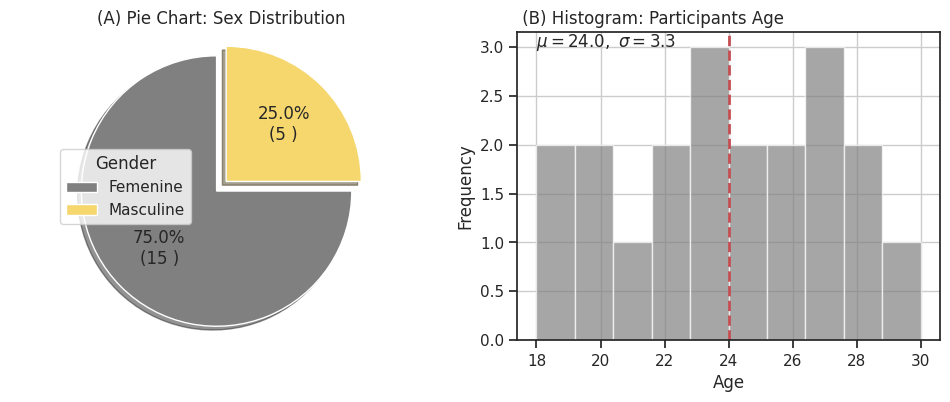
\includegraphics[width=15cm]{/home/perdices/Dokumente/Github/m-b_thesis/HU Thesis/figures/participants.png}
    \captionsetup{justification=justified, margin={2cm,2cm}, font={small}}
    \caption{After cleaning the data the study included 20 participants (\(\mu\)=24. years, \(\sigma\) = 3.3). As self-reported, all participants had normal vision, and no history of hearing loss or mental or neurological disorders, as self-reported. Notably, more women (15) responded to the call compared to men (5).}
    \label{fig:mesh1}
\end{figure}

    
\subsection*{Materials}

\subsubsection*{Electrocardiogram (ECG):}
Heart rate data was collected using an Arduino Uno and a SparkFun Single Lead Heart Rate Monitor - AD8232. The data was transferred through a USB 2.0 connection and integrated into the Unity log file at a frequency of 133 Hz. Compared to a clinical ECG, this device entails a serial interface that can send triggers via USB directly to a computer and software (e.g. Unity, Matlab) with minimal delay due to its architecture. Its software and hardware are open-source and publicly available \parencite{TimsECG}.

\subsubsection*{Head Mounted Display \& Lighthouses:}
The VR setup included a HTC Vive head-mounted display (HMD) with two lighthouses. The headset specifications included a Dual AMOLED 3.6" diagonal display, with 1080 x 1200 pixels per eye (2160 x 1200 pixels combined), a 90 Hz refresh rate, and a 110-degree field of view. The lighthouses are equipped with SteamVR Tracking, G-sensors, gyroscopes, and proximity sensors. Both the HMD and lighthouses are connected using USB 2.0. For this study, the VR controllers were not used, and instead, hand tracking was performed using the Leap Motion sensor.

\subsubsection*{Leap Motion Controller:}
This device was used to track the position of the hands. The Leap Motion Controller has a field of view of 150x120 degrees, with a variable range of roughly 80 cm (arm's length). It weighs 32 grams and is mounted on the HMD. The device features two 640x240 infrared cameras with a frame rate of 120 fps.

\subsubsection*{Haptic Data Gloves:}
The data gloves used in the study are equipped with magnetic sensors and connected to Unity using a micro USB connection. These gloves provide haptic feedback through 10 vibrotactile actuators, offering a wide range of tactile sensations with 1,024 levels of intensity. The gloves also incorporate complete finger tracking using six 9-axis Inertial Measurement Units (IMUs). These IMUs enable precise tracking of finger movements, allowing for accurate gesture recognition and enhanced interaction in virtual environments. The datagloves and finger tracking were interfaced from the experimental code using the \textit{UnityDll.Motion} and \textit{C\#} NeuroDigital licensed code (NeuroDigital Technologies, 2018).


\subsection*{Task}

In the following, I describe all tasks performed by participants. It's important to note that I didn't utilize all tasks from the original study. Nevertheless, considering that all included participants completed all questionnaires and tasks, the following description encompasses all tasks for transparency.

\textbf{Questionnaires:} Before the IVR experience, participants completed the Edinburgh Handedness Questionnaire to determine their handedness. The PRE-Cybersickness Questionnaire and POST-Cybersickness Questionnaire were administered before and after the IVR task to assess sickness symptoms in participants. Following the IVR experience, participants filled out the Virtual Reality Subjective Evaluation Questionnaire, designed to gather their perceptions of immersion, particularly considering tactile stimuli. 

\textbf{Heartbeat Count Task (HCT):} Participants performed a one-minute heartbeat count task before and after the IVR task. \footnote{Note that this task is not considered within this thesis due to being outside the scope of this secondary study.}

\textbf{IVR Memory-Motor Task:} 
After completing the initial questionnaires and HCT, participants moved to another room where the IVR equipment was set up. As mentioned this included a head-mounted display, data gloves, and an ECG device. 
For the implementation of the experiment, we used the Unity software (v2018.3.11; Unity Technologies, San Francisco, United States)  in combination with the SteamVR Unity plugin (Valve Corporation, Bellevue, United States). To synchronize the data streams (i.e., behavioural reports, hand positions, finger positions, ECG), we used custom C\# scripts and network-based communication (i.e., timestamps). 

The tactile stimuli was an activation of 10 vibrotactile actuators for 100 ms. The intensity of a vibrotactile pulse used in haptic feedback ranges from 0.0 to 1.0. The set intensity for the program was 0,2 as coded in Unity Game Engine. All levels had a maximal time of 2 minutes but all participants finished levels before the cap time by placing the ball before. The parameters, types, and spatial aspects of haptic feedback are configurable, allowing for a versatile setup suitable for psychophysical studies.

The virtual environment simulated a rectangular office with a window. Participants appeared sitting in front of a table. Just over the table, there is an initial prompt indicating them to place their hands over the table. 

In Figure \ref{fig:looks} are two panels. On the left side of the figure (Panel I), we observe the external view of a participant wearing the head device, ready to commence the IVR Memory-Motor Task. Panel II on the right side of the figure showcases four out of the five steps participants undergo when initiating a trial set. The steps are outlined below:

\begin{enumerate}
    \item[\textbf{a.}] Participants stand in front of a virtual table, allowing ample time to acclimate to the virtual environment, as depicted in Figure \ref{fig:looks}. When they feel prepared, the session commences as they calibrate by placing their hands on the virtual table.

    \item[\textbf{b.}] Before each trial within every set, a new calibration process begins. Participants place their palms facing up within the shadowed hands, ensuring standardized positioning. Refer to Figure \ref{fig:looks}b for the calibration setup.
    
    \item[\textbf{c.}] Once the calibration is complete, a two-dimensional sketch appears in front of them (Figure \ref{fig:looks}c), prompting them to memorize the red ball's position. Participants then observe a template on the table, resembling the initial sketch they memorized. Their task is to place the ball swiftly and accurately in the correct location on the template. In the memory sketch, the relevant position of the ball is denoted by the red circle. During this phase, participants keep their virtual hands open with palms facing up.
    
    \item[\textbf{d.}] As soon as the memory sketch disappears, a red ball appears in either the left or right hand of the participants. Simultaneously, a vibration could start in the glove. The vibration may or may not match the visual location of the red ball. If the vibrating hand matches the visual location of the ball,  the visual condition matches the tactile condition (V = T) and therefore the trail is congruent. If the vibrating hand does not match the visual location of the ball, then the visual condition does not match the tactile condition and the trial is incongruent ($V \neq T$). If there is no vibration at all, the trail condition is purely visual ($V$).
   
    \item[\textbf{e.}] After placing the ball on the template, the ball and template disappear. The whole process from (b) to (e) repeats.
\end{enumerate}


\begin{figure}[!ht]
    \centering
    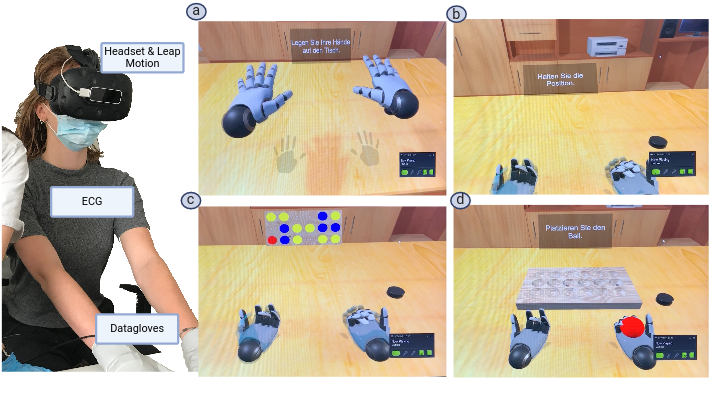
\includegraphics[width=15cm]{/home/perdices/Dokumente/Github/m-b_thesis/HU Thesis/figures/set_up_design.png}
    \put(-420,240){\textbf{I}} % Adjust (-20,340) to position "I" label as desired
    \put(-320,240){\textbf{II}} % Adjust (360,340) to position "II" label as desired
    \captionsetup{justification=justified, margin={2cm,2cm}, font={small}}
    \caption{IVR Memory-Motor Task: Panel I shows a participant wearing equipment. Panel II shows the different stages of one trial. (a) participants first view. Here they are asked to place the hands in the virtual table to start the calibration process. 2 seconds after placed the screen changes; (b) the second calibration phase adjusts wrists and fingers. 2 seconds after successfully superposing the hands in the signaled position the screen changes (c) while holding this position, participants are presented with a display of a 2D sketch for memorizing ball position for three seconds; (d) red ball is introduced in either hand an equal amount of times. Also the 3D template for ball placement ppears on the table marking the beginning of each trial.}
    \label{fig:looks}
\end{figure}
 
In a sequence of 105 trials, three conditions—congruent ($V=T$), incongruent ($V \neq T$), and visual-only ($V$)—were presented randomly and rapidly, each occurring 35 times. Each trial commenced upon positioning the ball in a hand, concluding only upon its precise placement on the designated template (refer to Figure \ref{fig:looks}). 

Given that an IVR task inherently involves proprioceptive signals, all conditions in the experiment integrate these signals and are thus multimodal. Consequently, the 'visual only' condition doesn't align with the unimodal classification commonly used in psychophysics literature. Nonetheless, for the sake of easier comparison to this literature in this thesis, I will refer to it as unimodal, and the congruent and incongruent conditions as bimodal.

\subsection*{Measures}
\subsubsection*{Immersive Virtual Reality (VR):}

Movement data from 3 devices was recorded (data gloves, Leap Motion device, and the HMD was collected). For movement analysis, only the wrist movements tracked by the Leap Motion device were considered, excluding the fingertips' magnetic tracking sensor data. All movements were recorded in an Euclidean coordinate system (X, Y, Z) with the original calibrating point set at (0, 0, 0). As each device had three coordinates, this provided a total of nine streaming sources of data (e.g., Headset X, Headset Y, Headset Z, and so on). Additionally, rotational data was recorded. Both sources are not included in the analysis since at the moment it does not help to compare with the race inequality model. 

Additionally, in the game output data, there are flags that signal if a button was pressed, if the ball is placed in the holder, and when the trial started. Trials where the error button was pressed were excluded from the analysis.

\subsubsection*{Questionnaires:}
Both of the described questionnaires are included in the appendix of this thesis for further reference. Questionnaire validation is outside the scope of this thesis:

\begin{enumerate}
\item[(i)] \textbf{Virtual Reality Subjective Evaluation Questionnaire:} This self-designed questionnaire comprises 26 items aimed at assessing the sense of reality experienced during the VR session. It explores factors like engagement level, hand movement, task difficulty, and other controlling aspects. Participants responded using a Likert scale rating them on a scale from 1 (Does Not Apply) to 7 (Totally Applies). The questions were organized in groups and inverted to confirm participants' responses. Both questionnaires can be found in the Appendix section.

\item[(ii)] \textbf{PRE/POST-Cybersickness Questionnaire:} This study employs a shortened version of the simulator sickness questionnaire \parencite{avpsy}. It utilizes a Likert scale ranging from one to four, featuring labels such as "not present," "somewhat," "clearly," and "very strongly." The questionnaire consists of 16 items, gauging symptoms like "fatigue" and "general discomfort," among others.
\end{enumerate}

\subsection*{Data Analysis}

\subsubsection*{Descriptive Statistics of the Subjective Evaluation}
The analysis of the questionnaire responses aimed to explore the impact of haptic gloves on reported immersion and related perceptions. Initially, raw questionnaire data were collected from 20 respondents, consisting of 27 questions rated on a scale from 1 to 7. Some participants did not answer all questions, thus creating specific missing values that were omitted. Statistical analysis included the calculation of descriptive statistics such as median ($\text{Mdn}$), mean ($\mu$), and standard deviation ($\sigma$) for each question. These statistics were instrumental in understanding the central tendencies and variability in respondents' perceptions. A full view of all answers can be found in the Supplements section.

\subsubsection*{Response Time preprocessing and analysis to test haptic glove condition}

Response times were calculated based on the interval between the virtual ball entering the scene and its disappearance. Trials where the error button was pressed were excluded from the analysis. Prior to analysis, outliers were identified and corrected by removing data points deviating more than 3 times the median absolute deviation (MAD), equivalent to 3 standard deviations assuming a normal distribution \parencite{Innes2019ACA}. No response times were excluded on account of being too fast; however, 13\% of trials were excluded due to excessive slowness. The final dataset comprised 1826 response times, approximately 24 per condition per participant. Following outlier removal, the response times for each condition were transformed into rates ($1/RT$).

The transformation method entails the inversion of the RT and aligns with prior studies \parencite{Innes2019ACA}. However, this transformation method is not exempt from criticism \parencite{Lo2015-fv}. This study prioritizes normality in error distribution over other factors such as property scale or interacting effects. This prioritization allowed for the direct application of repeated measures ANOVA within subjects. Yet, when the ANOVA results were ambiguous, a General Linear Mixed-Effect Model (GLMM) was additionally applied, as recommended by \textcite{Lo2015-fv}. By using GLMM, instead of imposing normality and eliminating error deviation, we allow the use of distributions that match the properties of the measured RT \parencite{Lo2015-fv}. I utilized the \textit{statsmodels} statistical package in Python, specifically the \textit{mixedlm} function, similar to other studies \parencite{RSE_FBI}. Although this analysis is not present in the reference study, the utilization of GLMM aims to provide clarity regarding the significance of the conditions and the study's power.

\subsubsection*{Cumulative Distribution Function and Race Model Inequality}

The Race Model statement is simple. It suggests that two different unimodal stimuli (e.g., vision, and touch) undergo processing in distinct sensory channels and race to trigger detection. If these two stimuli were presented simultaneously, then we would expect the fastest one to elicit the response (essentially, the one "winning the race"). Therefore, we would be right to expect inequalities (1) and (2) to be held:

\[
F_y(t) \leq F_x(t), \quad t > 0, \quad (1)
\]
\[
F_z(t) \leq F_x(t), \quad t > 0, \quad (2)
\]

A violation of the inequalities would require that two modalities presented at the same time have a faster response time than one of these modalities presented alone. This would indicate that the two modalities interacted in some way, thus explaining the faster response than a single modality on its own. Accurate knowledge of this is basic for understanding multisensory integration better.

Here, $F_x$ represents the cumulative density functions (CDFs) of reaction times (RT) in the individual stimulus conditions visual-only ($V$), respectively, while $F_y$ and $F_z$ denote the CDF of RT in the redundant-stimulus conditions congruent ($V=T$) and incongruent ($V \neq T$). According to race models, there's a possibility for $F_z(t)$ or $F_y(t)$ to closely approach $F_x(t)$ for small values of $t$, particularly in scenarios with strongly negative correlations in detection times \parencite{Ulrich2007}. However, even under these circumstances, the inequality must still hold as per the race models.

It is important to mention here that IVR does not allow the same experimental methodology as traditionally held in race model inequality studies. For example, a constant proprioceptive signal is inherent in the IVR design across all conditions, thus making absolute single modality impossible. Additionally, having only one single unimodal stimulus (vision) available prevents us from constructing the complete set of cases (single touch, single vision). Nevertheless, I make comparisons between the congruent and incongruent conditions with the single modality condition ($V$) based on the fact that they all have proprioceptive modality included, thus cancelling the effect out. Furthermore, constructing cumulative distribution functions allows for testing the statistical significance of these differences.

The process involved generating empirical cumulative density functions (CDFs) for three conditions—Bimodal pairs and Single Signal—and followed the steps outlined in literature \parencite{Ulrich2007}. The first steps were followed for every participant and every stimulus condition. Specifically, let $G_x$ be the individual CDF estimate of the visual-only condition, and $F_y$ and $F_z$ denote the redundant CDF for the incongruent and congruent conditions.

Consider a scenario where a set $\{x_1, x_2, \ldots , x_n\}$ of $n$ reaction times (RTs) has been recorded within condition $V$ for a specific participant. Arranging this sample in ascending order, from the smallest value to the largest—$x_1 \leq x_2 \leq \ldots \leq x_n$—one creates a step function. The second step involves using a step function to generate a cumulative frequency polygon. The final step is the estimation of percentiles and aggregation across participants. For a comprehensive breakdown and reference code, consult \cite{Ulrich2007}. Additionally, the code for this thesis is shared on GitHub.

To mimic the results from our reference paper \Cite{SALTAFOSSI2023108642}, I conducted a series of t-tests using individual participant data for the $F_x$, $F_y$, and $F_z$ values at each percentile level. Rather than examining areas under the curve, I focused on the raw values of $F_x$, $F_y$, and $F_z$. Furthermore, instead of emphasizing time bins, I opted to discuss percentile levels, given the differing time ranges compared to traditional RMI literature are longer because of answering times in IVR task.

\section*{3.Results}
\subsubsection*{Comparison of Cybersickness Levels Before and After Task, Alongside Subjective Evaluation Descriptive Statistics}

We conducted a paired-sample t-test to compare cybersickness levels before (Pre) and after (Post) the Virtual Reality Experience. Significant difference was found between Pre (M=1.10, SD=0.12) and Post (M=1.18, SD=0.19) conditions; $t(21)=-2.65$, $p = 0.015$, indicating symptoms transitioned from "not present" to "somewhat present".

Nineteen respondents answered 27 questions on the Virtual Reality Subjective Evaluation Questionnaire, rating them from 1 (Does Not Apply) to 7 (Totally Applies).

The haptic gloves were perceived to enhance the experience, with question 24 scoring "Applies" for perceived immersion ($\text{Mdn} = 6$, $\mu = 6$, $\sigma = 0.76$), and question 19 also rated as "Applies" for task enjoyment ($\text{Mdn} = 6$, $\mu = 5.4$, $\sigma = 1.04$).

However, haptic feedback was perceived as having a "Neutral" effect on performance (question 26: $\text{Mdn} = 3$, $\mu = 3.6$, $\sigma = 1.49$), response time (question 12: $\text{Mdn} = 3$, $\mu = 3.7$, $\sigma = 1.74$), and results (question 7: $\text{Mdn} = 6$, $\mu = 6$, $\sigma = 0.76$).

The memory task was generally perceived as easy, with disagreement on the difficulty of remembering the red ball's position (question 8: $\text{Mdn} = 5$, $\mu = 5.1$, $\sigma = 1.37$).

Question 13 about haptic feedback possibly eased ball placement showed high variance($\text{Mdn} = 5$, $\mu = 4.2$, $\sigma = 1.79$), then the "rather applies" is to be taken carefully.

Overall, participants reported increased immersion and enjoyment with the added gloves, but no perceived performance enhancement. Variations in responses to the last two questions suggest uncertainty about task ease. For detailed breakdown, please refer to the supplementary section.

\subsubsection*{Examining the Impact of Haptic Glove Stimuli on Response Time}

Initially, I assessed the mistake rates in ball placement (balls placed in a different position than the one qued in the prompter) across different conditions to ensure their negligible impact on the experiment. The mistake rates were as follows: in the visual-only condition ($V$), it was $6.35\%$ ($\pm 0.99\%$, SEM); in the visual incongruent touch condition ($V \neq T$), it was $5.79\%$. Additionally, a one-way ANOVA indicated no significant effects ($ F \leq 0.08$, $p \geq 0.91$) between all three experimental conditions (congruent, incongruent and visual-only). This task is considerably more complex than a simple yes-no detection task. Therefore, to some extent, we anticipate a higher mistake rate. Nevertheless, these rates remain notably low and were not subjected to further analysis.

To investigate whether the experimental manipulations successfully affected the RT, I conducted a one-way repeated-measures ANOVA. The test revealed a significant main effect for the stimulus ($F(2,38) = 3.4$, $p \leq 0.043$, $\eta p^2 = 0.15$). The median response time for the 'Congruent' condition ($V=T$) was the fastest ($3236$ ms $\pm 456$ ms), followed by the 'Incongruent' ($V \neq T$) condition ($3268$ ms $\pm 470$), while the slowest was observed in the absence of haptic stimuli 'None' ($V$) ($3284$ ms $\pm 463$). Thus, the experimental conditions significantly influenced response times, as illustrated in Figure \ref{fig:error}. However, post hoc Tukey HSD tests did not reveal any specific pairwise differences. While an overall difference among conditions was observed, specific pairwise differences were not identified.

\begin{figure}[!ht]
    \centering
    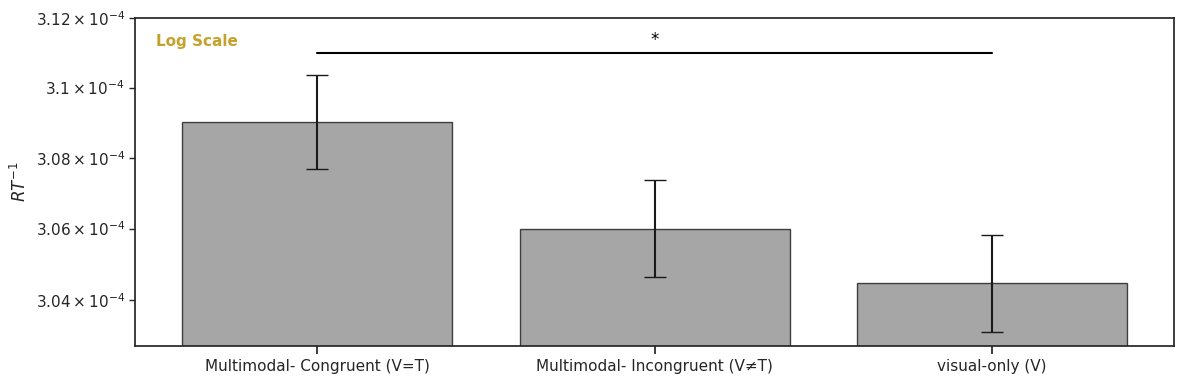
\includegraphics[width=15cm]{/home/perdices/Dokumente/Github/m-b_thesis/HU Thesis/figures/bar_erros_bars_stimulus_constructions.png}
    \captionsetup{justification=justified, margin={2cm,2cm}, font={small}}
    \caption{Passive haptic stimulus effect on RT. Boxplot of a One-way repeated-measures ANOVA using \(RT^{-1}\). The test revealed a significant main effect for the conditions (\(F(2,38) = 3.4\), \(p \leq 0.043\), \(\eta p^2 = 0.15\)).
    }
    \label{fig:error}
\end{figure}

Given the absence of identified specific pairwise differences in the post hoc analysis, I conducted a more comprehensive investigation using a Generalized Linear Mixed Model (GLMM).
The linear mixed model analysis aimed to assess the impact of conditions (($V=T$), ($V \neq T$), ($V$)) on response times. The model included condition as a fixed effect and participant as a random effect, with the 'Congruent' condition serving as the reference category.

Although this specific analysis method was not employed in the referenced paper \parencite{SALTAFOSSI2023108642}, it offers numerous advantages for multilevel research designs. It addresses, for example, the issue of the linear relationship between the standard deviation of RT and mean RT, characterized by an increasing spread in residuals for longer predicted RT \parencite{Lo2015-fv}.

The model coefficient for the 'None' ($V$) condition ($\beta = 45.726, SE = 22.594, p = 0.043$) reached statistical significance at the conventional level ($\alpha =0.05 $) when compared to the 'Congruent' ($V=T$) condition. This suggests a significant difference in response times between the 'None' and 'Congruent' conditions. The coefficient for the 'Incongruent' condition ($\beta = 32.975, SE = 22.686, p = 0.146$) did not reach conventional levels of significance. 

Thus, the 'Congruent' condition demonstrated significantly faster performance compared to the visual-only condition. This outcome aligns with the expected results according to the RSE. However, the findings present a mixed perspective. Despite this significant contrast, the more stringent post hoc Tukey HSD tests revealed no notable differences between pairwise conditions. Additionally, the GLMM indicated significance solely between the 'Congruent' ($V=T$) and visual-only ($V$) conditions and not between the 'Congruent' ($V=T$) and 'Incongruent' ($V \neq T$) conditions. We should consider that median time differences between conditions range between 30 to 50 milliseconds. Now that we have validated the condition. To gain a deeper understanding of the results and nest them in the literature the next section of RMI and CDF analysis will aim to achieve this. 

\subsubsection*{Cumulative Distribution Functions Race Model Inequeality}

In this section, I utilize the Cumulative Distribution Function (CDF) from the Race Model Inequality (RMI) model to evaluate the significance between conditions at different time points ($t$). The t-test conducted between the three experimental conditions revealed significant differences between the 'Congruent' and visual-only ($V=T$ ; $V$) conditions, but no significant differences emerged between the 'Congruent' and 'Incongruent' conditions ($V=T$ ; $V \neq T$). The results between $F_x$ and $F_z$ ($V$ ; $V=T$) are presented in Table \ref{tab:response-time-range}, which illustrates the results for all time frames and percentiles. Notably, significant differences emerged between $F_x$ and $F_y$ from the 16th percentile onwards. Interestingly, for this percentile (as depicted in Figure \ref{fig:CDF}), the single modality visual ($V$) appears to be faster than the bimodal incongruent condition ($V \neq T$), suggesting a potential violation of the RMI principle. Conversely, from the 40th percentile onwards, both redundant signals consistently demonstrate faster response times compared to the unimodal signal, aligning with our expectations based on the RSE. It's important to note that when considering the distribution of all response times, the highest density is observed between 3100 and 3200 ms, accounting for 33\% of all response times.

\begin{table}[!ht]
    \centering
    \adjustbox{max width=\textwidth}{
    \begin{tabular}{ccccccccc}
    \hline
    \textbf{Percentile Estimation} & \textbf{$F_z$ Time Range (ms)} & \textbf{$F_z$ Min Max Diff (ms)} & \textbf{$F_z$ T-value} & \textbf{$F_z$ p-value} & \textbf{$F_y$ Time Range (ms)} & \textbf{$F_y$ Min Max Diff (ms)} & \textbf{$F_y$ T-value} & \textbf{$F_y$ p-value}  \\ \hline
    10 & (3070, 3621) & 551 & 1.19 & 0.12 & (3121, 3907) & 786 & 1.1 & 0.14 \\
    13 & (3078, 3626) & 548 & 1.31 & 0.1 & (3123, 3969) & 846 & 0.79 & 0.22 \\
    16 & (3084, 3648) & 564 & 1.88 & 0.04* & (3130, 4171) & 1041 & 0.92 & 0.18 \\
    19 & (3086, 3687) & 600 & 2.04 & 0.03* & (3141, 4352) & 1211 & 0.96 & 0.18 \\
    20 & (3087, 3708) & 621 & 2.01 & 0.03* & (3153, 4645) & 1492 & 0.96 & 0.17 \\
    23 & (3092, 3748) & 656 & 1.97 & 0.03* & (3176, 4948) & 1772 & 0.99 & 0.17 \\
    26 & (3094, 3760) & 665 & 2.06 & 0.03* & (3202, 5060) & 1857 & 1.04 & 0.16 \\
    29 & (3098, 3766) & 668 & 2.03 & 0.03* & (3221, 5184) & 1963 & 1.33 & 0.1 \\
    30 & (3099, 3768) & 668 & 2.02 & 0.03* & (3241, 5290) & 2049 & 1.34 & 0.1 \\
    33 & (3104, 3814) & 709 & 2.11 & 0.02* & (3264, 5391) & 2127 & 1.02 & 0.16 \\
    36 & (3106, 3838) & 732 & 2.08 & 0.03* & (3287, 5558) & 2271 & 0.95 & 0.18 \\
    39 & (3111, 3846) & 735 & 1.83 & 0.04* & (3311, 5739) & 2427 & 1.13 & 0.14 \\
    40 & (3114, 3848) & 734 & 1.79 & 0.04* & (3336, 5884) & 2548 & 1.19 & 0.12 \\
    43 & (3119, 3861) & 741 & 1.74 & 0.05* & (3361, 6067) & 2706 & 1.16 & 0.13 \\
    46 & (3121, 3907) & 786 & 1.55 & 0.07 & (3396, 6271) & 2946 & 0.85 & 0.2 \\
    49 & (3123, 3969) & 846 & 1.36 & 0.09 & (3431, 6503) & 3181 & 0.48 & 0.32 \\
    50 & (3124, 3978) & 855 & 1.33 & 0.1 & (3466, 6723) & 3421 & 0.29 & 0.39 \\
    60 & (3130, 4171) & 1041 & 1.25 & 0.11 & (3499, 6989) & 3680 & 0.91 & 0.19 \\
    70 & (3141, 4352) & 1211 & 1.21 & 0.12 & (3530, 7310) & 3939 & 0.4 & 0.35 \\
    80 & (3153, 4645) & 1492 & 1.47 & 0.08 & (3560, 7674) & 4253 & -0.54 & 0.7 \\
    90 & (3176, 4948) & 1772 & 0.53 & 0.3 & (3589, 8081) & 4632 & -0.27 & 0.61 \\ \hline
    \end{tabular}}
    \captionsetup{justification=justified, margin={2cm,2cm}, font={small}}
    \caption{Each row is organized around a percentile estimated for the cumulative distribution function (CDF). The estimations were made for each participants RT indiviually and then grouped together around percentile. The column "Time Range (ms)" shows the fastest and slowest RT for the percentile group. The column "difference" indicates the difference between the minimal and maximal response time. Both conditions, $F_y$ (bimodal-incongruent) and $F_z$ (bimodal- congruent) are compare to visual-only $G_x$ in a single-side t-test.}
    \label{tab:response-time-range}
\end{table}


\begin{figure}[!ht]
    \centering
    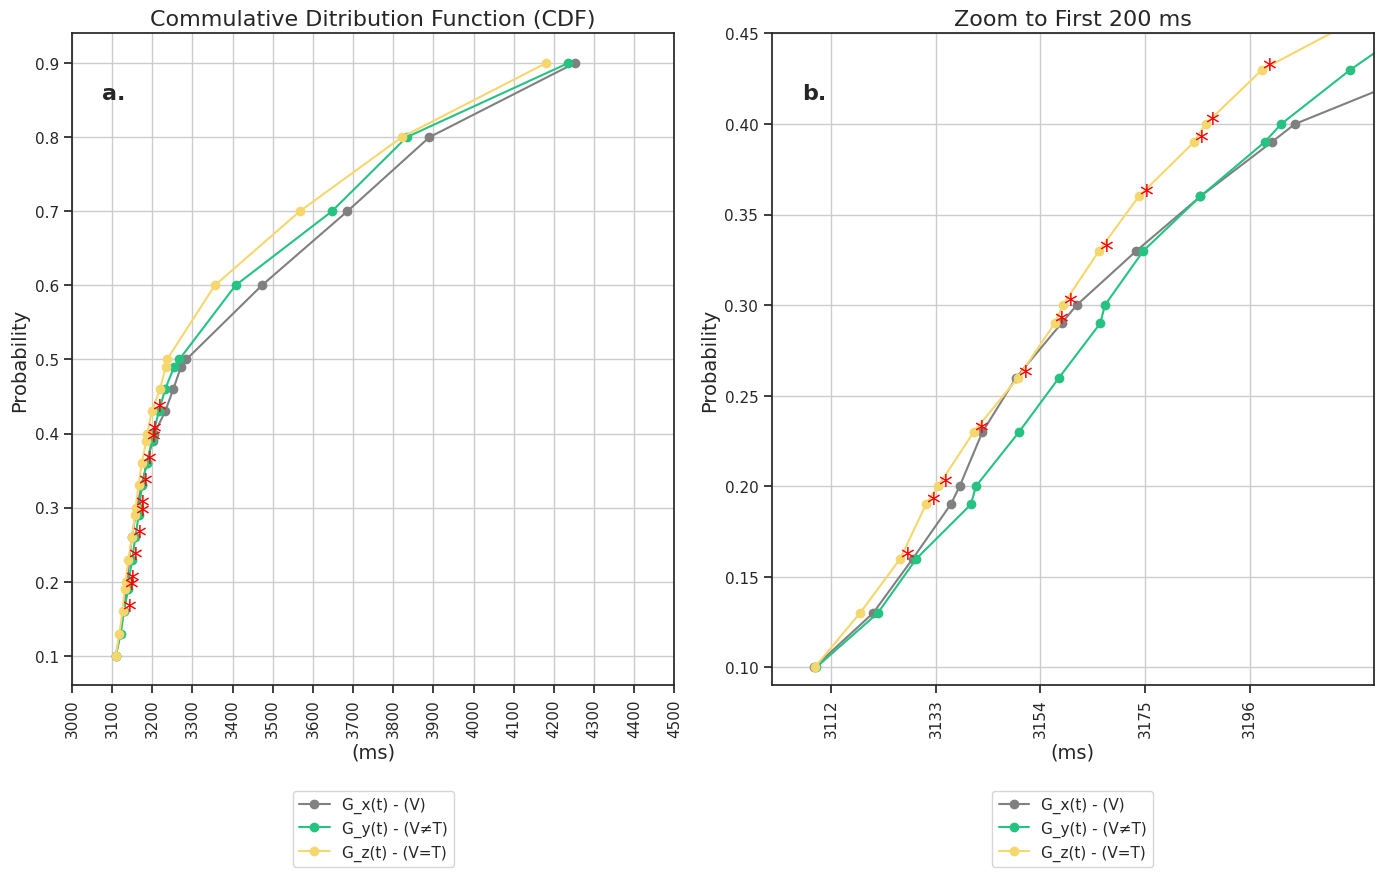
\includegraphics[width=\textwidth]{/home/perdices/Dokumente/Github/m-b_thesis/HU Thesis/figures/CDF.png}
    \captionsetup{justification=justified, margin={2cm,2cm}, font={small}}
    \caption{ Cumulative distribution functions F(t) of RTs for $F_y$ (bimodal-incongruent) and $F_z$ (bimodal- congruent) and visual-only $G_x$. (a.) Displays the estimated percentile points for each of the three functions of interest: $G_x$, $F_y$, $F_z$, considering all participants. 
    (b.) Is a zoom in the first 100 ms of the entire RT range. Acording to the RSE, the CDF $G_x$ of the visual-only ($V$) condition should be under $F_y$, $F_z$ at all moments. Our data shows that is not the case for the first 100 ms of the entire RT range.}
    \label{fig:CDF}
\end{figure}


\section*{4.Discussion}

In this study, I examined whether an experimental setup using IVR and haptic gloves could reproduce established practices in multisensory integration, drawing from previous research data. Specifically, I focused on psychophysical experimental configurations that evaluate Miller's inequality. Additionally, I capitalized on the discrepancy between haptic gloves and real-life experiences to investigate the impact of congruency on multisensory integration. The findings not only confirm the utility of IVR in studying multisensory integration but also offer a pathway to merging insights from psychophysics and cognitive research into a unified framework. Furthermore, preliminary results prompt inquiry into the role of higher-order congruency, such as "feeling touch where we see it," in early integration processes extending beyond temporal and spatial congruencies.

%The study employs a within-subject experimental design, using as manipulation the haptic feedback of the glove. Within the virtual environment, the task required the participants to watch for 3 seconds and remember the correct within 18 positions to place the ball from a prompter. As the ball is placed in the hand of the participants they are required to place as fast as possible in the 3D template in front of them. 

%The condition was designed so that a passive vibrotactile stimulus is activated when a red ball visually appears in the hand. When there is a match between the visual location of the ball and the vibration of the glove, then it's called congruent visual-tactile stimuli ($V=T$). When there is a mismatch between the location of the ball and the vibration of the glove, then it's called incongruent visual-tactile stimuli ($V \neq T$). Finally, when there is no vibration in any glove but only IVR visual cues, then the condition is called visual-only stimuli ($V$). 

To validate the construction of stimuli, I analyzed and modeled the reaction times across congruent, incongruent, and visual-only conditions. In total, more than a third of the trials yielded responses within the narrow timeframe of 3100 to 3200 milliseconds from the onset. While the ANOVA results unveiled a significant overall difference among all conditions, attempts to pinpoint specific pairwise distinctions using a Tukey HSD test yielded no significant findings. However, a GLMM analysis revealed a notable disparity between the visual-only ($V$) and visual-touch congruent ($V=T$) conditions. Interestingly, no significant differences were discerned between the incongruent ($V \neq T$) and visual-only ($V$) conditions.

When conducting a t-test, the RMI analysis reveals a significant discrepancy in the cumulative distribution functions (CDF) between the unimodal visual-only condition ($G_x$) and the bimodal congruent condition ($F_y$). Specifically, for $F_y$, this t-test identified a significant difference compared to the visual-only condition within the narrow time frame of 3100 to 3200 milliseconds (the initial 100 milliseconds), representing the period of highest response density. Notably, no significant differences were observed for the incongruent condition across any time period.

Descriptively, the relationship between the visual-only ($V$) and congruent condition ($V=T$) remains consistent across the entire range of reaction times (RT), aligning with the Race Model inequality (RMI). However, this pattern doesn’t hold for the RT relation between the incongruent condition ($V \neq T$) and the visual-only condition ($V$), where within the first 100 ms of the complete RT range, the unimodal condition displays faster responses than the bi-modal incongruent condition ($V \neq T$), potentially breaching the expected inequality. In later response times, the incongruent condition is faster than the unimodal visual-only condition, as anticipated. This, like in previous literature, again raises the question of a possible violation of the RMI model. Particularly as a bimodal condition ($V \neq T$) demonstrates faster responses compared to an unimodal condition ($V$).

However, as the statistical significance is a border value and the effects are relatively minor, I want to be cautious about the implications. Another study by \cite{RSE_FBI} investigating embodiment illusion (the reported feeling of seeing one body where it is not) yielded similar results concerning the irrelevance of stimuli for reaction times (RT). Their hypothesis suggests that the absence of a difference in the Race Model Inequality (RMI) between congruent and incongruent conditions could be due to the simultaneous occurrence of visual and vibrotactile stimuli. This simultaneous presence might suffice for multisensory integration, regardless of whether this crossmodal stimulus is functionally link at a higher level (e.g., touch in the hand holding the ball) \parencite{RSE_FBI}. Also, another relevent study looking to measure the effect of multisensory integration in VR on increasing performance in a task (e.g. hiting targets and duration) found that for the visual-touch condition only there is a increase in performance nontheless no reflected in P300 responses \parencite{Marucci2021TheIO}.  
%% up unitill here grammar correctedd.
I speculate that the data shows that the incongruent effect is outweighed by integration caused by the synchronicity of stimuli and sharing the same receptive field. It would be interesting to look further into this phenomena in future research especially since we remain largely ignorant of the areas of the human brain sensitive to semantic or contextual congruence between multiple sensory cues. 

\subsubsection*{Limitations}

Some of this study's limitations come from the fact that each trial in our IVR study spans a longer time frame when compared to traditional psychophysics experiments (with a mean duration of 3400 ms versus the typical 200 ms). This extended duration contributes to increased variance and skewness in reaction times (RT) as I addresed it. Nonetheless, it makes the comparison to previous studies harder.  Additionally, a new design should pay attention to the latencies between all interfaces (e.g., ECG, Gloves, HMD) and integrate them considering the latest proposed standardizations \parencite{vr_respont}. As mean differences between somatosensory conditions might be as small as 20 ms, latency integration issues over 7 ms might hinder the results. Furthermore, the programming of the experiment should give the researcher different cutoff moments in the experiment (e.g. movement initiation vs task completion) to have better control over the RT skewness and variance, thus avoiding the skewness problem and increasing the significance of the results. Previous research on RMI employs various methods to assess the significance of differences between conditions, yet more consensus on the most appropriate methods is needed. Additionally, future studies could benefit from larger sample sizes, such as involving 60 participants, to draw more definitive conclusions regarding the integratory enhancement effect of congruent stimuli, while considering the time effect on reaction time of 20 ms. 
\newpage
\begin{figure}[ht]
        \centering
        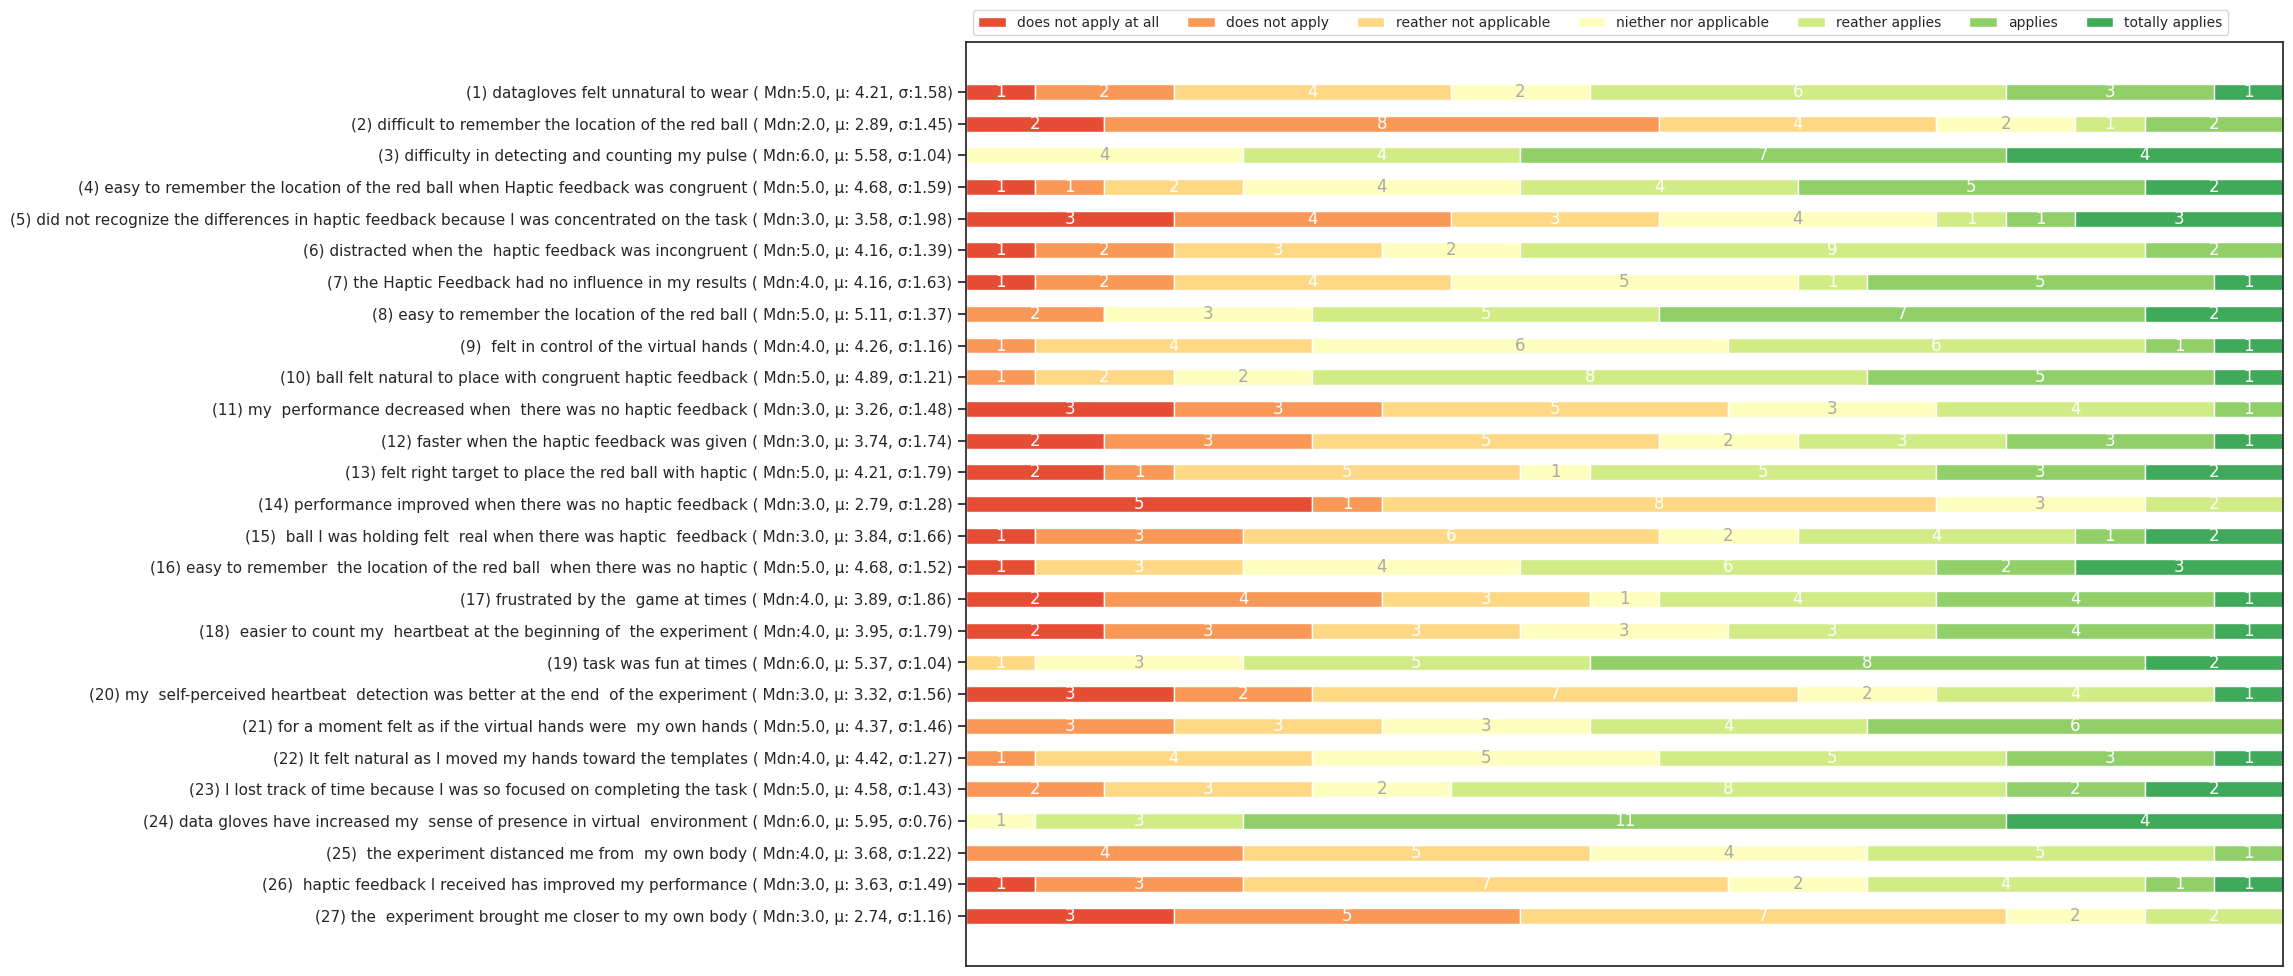
\includegraphics[angle=90, width=\textwidth, height=20cm, keepaspectratio]{/home/perdices/Dokumente/Github/m-b_thesis/HU Thesis/figures/questionaire_fig.png}
        \captionsetup{justification=justified, margin={2cm,2cm}, font={small}}
        \caption{Results: Virtual Reality Subjective Evaluation Questionnaire}
        \label{fig:quest}
\end{figure}
\pagebreak


%-------- CREATING BIBLIOGRAPHY

\paragraph{\textbf{References}}
\printbibliography[heading=none]

%-------- CREATING Apendix

\pagebreak
\vspace*{\fill}
\section*{\centering Additional Material}
\vspace*{\fill}



\end{document}

